\documentclass[xcolor=pdftex,dvipsnames,table]{beamer}
\usetheme{Boadilla}
\usecolortheme{crane}
\usepackage[utf8]{inputenc}
\usepackage[english]{babel}
\usepackage{amsmath}
\usepackage{amscd}
\usepackage{amsfonts}
\usepackage{amssymb}
\usepackage{graphicx}
\usepackage{pgfplots}
\usepgfplotslibrary{fillbetween}
\usepackage{centernot}
\usepackage{mathrsfs} % x \mathscr fonts 
\usepackage{bm}
\usepackage{soul,xspace}
\usepackage{marvosym}
\usepackage{tikz}
\usetikzlibrary{positioning}
\usepgflibrary{shapes.arrows}
\usetikzlibrary{shapes.geometric,mindmap,fit}
\usepgflibrary{shapes.misc}
\usetikzlibrary{shadows}
\usetikzlibrary{arrows}
\usetikzlibrary{calc}
\let\labelstyle=\textstyle
\pgfdeclarelayer{background} \pgfdeclarelayer{foreground}
\pgfsetlayers{background,main,foreground}
%\usetikzlibrary{backgrounds}

\usepgflibrary{decorations.pathmorphing}
\usepgflibrary{decorations.text}

\usetikzlibrary{calc,shapes.geometric,shapes.symbols}
\usetikzlibrary{shapes.callouts}
\usetikzlibrary{patterns}

% the following package is optional:
%\usepackage{latexsym} 

%%%%%%%%%%%%%%%%%%%%%%%%%%%%%%%%%%%%%%%%%%%%%%%%%%%%%%%%%%%%%%%%%%%%%%%%%%%%%%%%%%%%%%%%%%%%%%%%%%%

\def\wrt{wrt.\xspace}

\definecolor{yellow-dark}{rgb}{.9,.9,0}
%\definecolor{Light}{gray}{.80}
%\definecolor{Dark}{gray}{.20}
\newcommand<>{\gl}[1]{\only#2{\colorbox{Light}}{\only#2{\textcolor{Dark}}{#1}}}
\newcommand<>{\gd}[1]{\only#2{\colorbox{Dark}}{\only#2{\textcolor{white}}{#1}}}
\newcommand<>{\tbf}[1]{\only#2{\textbf{#1}}}
\newcommand<>{\redd}[1]{{\only#2{\color[rgb]{1,0,0}}#1}}
\newcommand<>{\bluee}[1]{{\only#2{\color[rgb]{0,0,1}}#1}}
\newcommand<>{\greenn}[1]{{\only#2{\color[rgb]{0,1,0}}#1}}
\newcommand<>{\grayy}[1]{{\only#2{\color[rgb]{.6,.6,.6}}#1}}

\def\red{\color[rgb]{1,0,0}}
\def\black{\color[rgb]{0,0,0}}
\def\gray{\color[rgb]{.6,.6,.6}}
\def\K{\texttt{K}}
\def\,{\texttt{,}}
%\def\'{\texttt{'}}
\def\*{\texttt{*}}
%\def\pgfline\alt<6>{\pgfsetlinewidth{1pt}}{\pgfsetlinewidth{.4pt}}
\newcommand<>{\lbf}{\alt#1{\pgfsetlinewidth{1pt}}{\pgfsetlinewidth{.4pt}}}
\newcommand<>{\lbff}{\alt#1{\pgfsetlinewidth{1.6pt}}{\pgfsetlinewidth{.7pt}}}
\def\ll{\pgfsetlinewidth{.4pt}}

\def\qed{ \hfill{$\Box$}}
\definecolor{Light}{gray}{.80}
\definecolor{Dark}{gray}{.20}
\def\gl#1{\colorbox{Light}{\textcolor{Dark}{#1}}}
\def\gd#1{\colorbox{Dark}{\textcolor{white}{#1}}}
\def\O{\mathcal{O}}
\def\Q{\mathcal{Q}}
\def\R{\mathcal{R}} % a mathematical relation
\def\S{\mathcal{S}}

\def\P{\mathcal{P}}
\def\F{\mathcal{F}}
\def\PP{\mathsf{\Pi}}
\def\I{\mathscr{I}}
\def\RF{R^{F*}} %a fuzzy instance of R
\def\QF{Q^{F*}} %a fuzzy instance of Q
\def\adr{\rm{adr}}
\def\PF{{\rm PF}}
\def\T{\mathcal T} %set of base types of attributes
%\def\Dom{\rm Dom}

\def\Int{\ensuremath{\I}}  % Interpretation
\def\IntP{\ensuremath{\I_\PS}}
\def\Q{\mathcal{Q}}
\def\DBR{\ensuremath{\bm{R}}} % DB schema R
\def\DBI{\ensuremath{\bm{I}}} % DB instance I
\def\DBS{{\ensuremath{\bm{S}}}} % DB schema S
\def\DBJ{{\ensuremath{\bm{J}}}} % DB instance J
\def\ATT{{\ensuremath{\bm{A}}}} % relation attributes


\def\eo{\mathrel{\accentset{\text{e}}{\sqsubseteq}}}
\def\SPM{\ensuremath{\mathscr{M}}}  % set of preference models
\def\PMWS#1{\ensuremath{\succeq^{\bm{W}}_{#1}}}
\def\DB{\ensuremath{\bm{D}}}
\def\I{\ensuremath{\mathscr{I}}}

\DeclareMathOperator\OPT{Opt} \DeclareMathOperator\dom{dom}
\DeclareMathOperator\PI{PI} \DeclareMathOperator\Inst{Inst}

 \def\EX1{Non-IR cameras shooting a lit gate area\xspace}
 \def\BR#1#2{\ensuremath{\left\langle #1,#2\right\rangle}}
 \def\PP{\ensuremath{\mathrel{\succeq}}}
 \def\NPP{\ensuremath{\mathrel{\nsucceq}}}
 \def\AW{{\ensuremath{\Omega}}} %acceptable world
 \def\PS{{\ensuremath{\mathcal{P}}\xspace}}
 \def\LP{\ensuremath{\mathcal{L}_{\PS}}}

\newdimen\radius

\def\mgm{\mathrel{{}^m\!\!>^m}}
\def\mgM{\mathrel{{}^m\!\!>^M}}
\def\Mgm{\mathrel{{}^M\!\!>^m}}
\def\MgM{\mathrel{{}^M\!\!>^M}}
\def\mgeqm{\mathrel{{}^m\!\!\geq^m}}
\def\mgeqM{\mathrel{{}^m\!\!\geq^M}}
\def\Mgeqm{\mathrel{{}^M\!\!\geq^m}}
\def\MgeqM{\mathrel{{}^M\!\!\geq^M}}
%\def\mgeqcm{\mathrel{{}^m\!\!\geq^m_c}}
%\def\mgeqcM{\mathrel{{}^m\!\!\geq^M_c}}
%\def\Mgeqcm{\mathrel{{}^M\!\!\geq^m_c}}
%\def\MgeqcM{\mathrel{{}^M\!\!\geq^M_c}}

\def\prm{{\ensuremath{\mathop{\pi}}}}


%%%%%%%%%%%%%%%%%%%%%%%%%%%%%%%%%%%%%%%%%%%%%%%%%%%%%%%%%%%%%%%%%%%%%%%%%%%%%%%%%%%%%%%%%%%%%%%%%%%

\def\MLN{MLN}
\def\HMLN{HMLN}
\def\hMLN{(H)MLN}

\def\VMLN{VMLN}
\def\SemCla{SemCla} % the prototype implementation
\def\RHS{RHS}  % right-hand side (of an equation)
\def\LHS{LHS}  % left-hand side (of an equation)
\def\wlg{w.l.o.g.} % without loss of generality
\def\Wlg{W.l.o.g.} % without loss of generality
\def\ae{a.e.} % almost everywhere
\def\wff{wff} % well formed formula
\def\KFA{known functions assumption} % a representation assumption 
\def\DCA{domain closure assumption} % a representation assumption 
\def\KF{known functions} 
\def\DC{domain closure} 
\def\UNA{unique names assumption} % a representation assumption

\def\Sorts{\ensuremath{\mathit{Sorts}}}
\def\Symbols{\ensuremath{\mathit{Symbols}}}
\def\type{\ensuremath{\mathit{type}}}
\def\Ind{\ensuremath{I}} % Indicator function

\def\Ar{\ensuremath{\mathit{Ar}}}
\def\DD{\ensuremath{D}}  % the domain of discourse of Interpretations
\def\Interp{\ensuremath{\mathcal{I}}} % Interpretation
\def\InterpD{\ensuremath{\Interp|_d}} % discrete part of an Interpretation
\def\InterpC{\ensuremath{\Interp|_c}} % continuous part of an Interp.
\def\AllInterp{\ensuremath{\mathscr{I}}} % th set of all Interpretations
\def\vel{\ensuremath{\mathrm{or}}} % semantical inclusive OR
\def\at{\ensuremath{\mathrm{and}}} % semantical AND
\def\xor{\ensuremath{\mathrm{xor}}} % XOR
\def\val{\ensuremath{v}} % valuation -- a truth value assignment
\def\HI{\ensuremath{H_\Interp}}  % Herbrand interpretation


\def\LL{\ensuremath{\mathcal{L}}}  % FOL language
\def\Theory{\ensuremath{\mathcal{T}}} % FOL theory
\def\nnconst{\ensuremath{a}} % a new non-numeric constant of \LL 
\def\ext{\text{\nnconst}}  % extension of \Theory: \Theory_\ext
\newcommand{\Theories}[1]{\ensuremath{\bm{\Theory}_{\!\!\!#1}}} % a vector of theories
\def\Tiid{\ensuremath{\Theory_1}}    % Theory_2
\def\Tiiid{\Theories{}}  % <\Theory_1,\Theory_2,\Obs>
\def\enumq{Q}  % enumerate Queries in compactenum, e.g., (Q-1.), (Q-2.), etc.
%\def\Theories{\ensuremath{\bm{\Theory}}} % a vector of theories
\def\NT{\ensuremath{\mathscr{D}}}  % numeric terms
\def\nt{\ensuremath{F}}  % a numeric term
\def\numTerm{dependence term}  % original numeric term
\def\NumTerm{Dependence term}  % original numeric term
\def\NumTERM{Dependence Term}
\def\numVect{dependence vector}  % dependence vector
\def\nVect{numeric vector}  % numeric vector
\def\OBS{\ensuremath{\bm{D}}}  % Observations: data with values \Obs
\def\Obs{\ensuremath{\bm{d}}}  % Observations - values
\def\rvect{\ensuremath{\vect{x}}} % vector of random variables
\def\yvect{\ensuremath{\vect{y}}} % vector of random variables

\def\Rvect{\ensuremath{\vect{X}}} % random vector
\def\Yvect{\ensuremath{\vect{Y}}} % random vector
\def\Rvar{\ensuremath{X}} % vector of random variables
\def\Zvect{\ensuremath{\vect{Z}}} % random vector
\def\Dom{\ensuremath{\mathrm{Dom}}} % Domain
\def\ArgMax{\mbox{\ensuremath{\mathrm{arg\, max}\;}}}
\def\Indep{\ensuremath{\perp\!\!\!\perp}}  % stochastic independence  


\def\M{\ensuremath{\mathcal{M}}} % A model (structure)
\def\MM{\ensuremath{\mathscr{M}}} % A set of models (structures)
\def\GG{\ensuremath{\mathscr{G}}} % A set of interpretations of function symbols
\def\h{\ensuremath{\bm{h}}}
\def\param{\ensuremath{\omega}}
\def\prm{\ensuremath{\bm{\param}}} % matrix of parameters of all PDFs
\def\Prm{\ensuremath{\bm{\Omega}}} % the domain of the matrix of parameters of all PDFs
\def\wfce{\ensuremath{h}}  % the function used in the Def. of weight function w = h()*w_i()


\def\OutcSpace{\ensuremath{\AllInterp}}  % sample (stat)/outcome (probability) space
\def\OutcSpaceR{\ensuremath{\widetilde{\AllInterp}}}  % sample (stat)/outcome (probability) space restricted by Representation Assumptions
\def\SigField{\ensuremath{\mathbb{I}}} % sigma-field
%\def\prmm{\ensuremath{\bm{\vartheta}}}
\def\MRF{\text{MRF}} % Markov random field 
\def\GRF{\text{GRF}} % Gibbs random field
\def\UndG{undirected graph}  % undirected graph
\def\Exp{\ensuremath{\mathds{E}}}  % expectation
\def\const{\text{const}} 
\def\N{\ensuremath{\mathcal{N}}} % Normal distribution
\def\bmu{\ensuremath{\bm{\mu}}}  %mean
\def\bsigma{\ensuremath{\bm{\sigma}}} % variance
\def\blambda{\ensuremath{\bm{\lambda}}} % precision
\def\bpi{\ensuremath{\bm{\pi}}}

\def\ba{\ensuremath{\bm{a}}} % vector of constants
\def\bz{\ensuremath{\bm{z}}}
%\def\beeta{\ensuremath{\bm{\eta}}}
%\def\bxi{\ensuremath{\bm{\xi}}}
\def\semcla{\textsf{SemCla}}
\def\R{\ensuremath{\mathds{R}}}   % reals
\def\Nn{\ensuremath{\mathds{N}}}   % natural numbers
\def\BB{\ensuremath{\mathcal{B}}}   % Borel sigma-field
\def\IndF{\ensuremath{\mathit{I}}}  % Indicator function

\def\countM{\ensuremath{P_c}}  % counting measure
\def\IcountM{\ensuremath{\nu_c}}  % induced counting measure
\def\LebM{\ensuremath{m}}  % Lebesgue measure


\def\Nat{\ensuremath{\mathds{N}}}  % Natural numbers
\def\bgamma{\ensuremath{\bm\gamma}}
\def\balpha{\ensuremath{\bm\alpha}}
\def\bw{\ensuremath{\bm{w}}}
%\def\bx{\ensuremath{\bm{x}}} % vector of variables
\def\BetaD{\ensuremath{\mathrm{Beta}}}
\def\Dir{\ensuremath{\mathrm{Dir}}}
\def\Gam{\ensuremath{\mathrm{Gam}}}
\def\nump{\ensuremath{\tau}}  % numeric property
\def\numpV{\ensuremath{\vect{\nump}}}  % vector of numeric properties
\def\numpS{\ensuremath{\bm{\nump}}}  % set of numeric properties

\def\Nump{\ensuremath{\vect{G}}}  % interpretation of num. properties 
\def\Clique{\ensuremath{\mathcal{C}}}  % clique in a graph
\def\WWeights{\ensuremath{\bm{\mathrm{U}}}} % a matrix of weights
\def\Weights{\ensuremath{\mathrm{U}}} % an element of a matrix of weights
\def\PPf{\ensuremath{\bm{\mathrm{P}}}} % matrix-valued function 
\def\Pf{\ensuremath{\mathrm{P}}} % an element of a matrix-values function

%\def\npf{\ensuremath{{\delta}}}  % numeric property function
%\def\ff{\ensuremath{s}}  % formula feature 
\def\feature{\ensuremath{\eta}} % eta
%\def\vv{\ensuremath{\mathbf{v}}}  % vector v
\def\RHS{RHS}  % right hand side
\def\Const{\ensuremath{\mathcal{O}}}  % set of constants
\def\T{\mathrm{T}}  % transposition (a superscript of a vector or a matrix)
\def\diag{\ensuremath{{\mathrm{diag}}}}  % diagonal matrix
\def\bphi{\ensuremath{\bm\phi}}  % N x K matrix of mixture coefficients 
\def\IND{\ensuremath{\mathds{1}}}
\def\I{\ensuremath{\bm{\mathrm{I}}}}  % Identity matrix

\def\PDF{PDF}  % probability density function
\def\CDF{CDF}  % cumulative distribution function
\def\cdf{\ensuremath{\mathcal{P}}}  % cumulative distribution function
\def\pClique{\ensuremath{p_\Clique}} % \PDF of isolated Clique
\def\MAP{\text{MAP}}

\def\defined{\overset{\vartriangle}{=}}  % := 

\newcommand{\comm}[1]{}  % to comment out a few words in the middle of a row
\newcommand{\vcr}[1]{\ensuremath{\overrightarrow{#1}}} % vector with an arrow
\newcommand{\vect}[1]{\ensuremath{\mathbf{#1}}}       % vector without an arrow
%\def\PDFprm{\ensuremath{\vcr{\theta}}} 
\newcommand{\PDFprm}[1]{\ensuremath{\vcr{\theta_{#1}}}}
\newcommand{\Ran}[1]{{\ensuremath{\mathrm{Ran}{\,#1}}}}  % Range of a function


\def\ones{\ensuremath{\vect{1}}}  % all-ones vector

\newcommand{\exend}{\hfill \ensuremath{\triangleleft}}
\newcommand{\remend}{\hfill \ensuremath{\diamond}}
\newcommand{\defend}{\hfill \ensuremath{\diamond}}

%\theoremstyle{definition}
%\newtheorem{definition}{Definition}
%\newtheorem{example}{Example}

%\theoremstyle{remark}
%\newtheorem{remark}{Remark}

%\theoremstyle{plain}
\newtheorem{hypothesis}{Hypothesis}
%\newtheorem{proposition}{Proposition}
%\newtheorem{theorem}{Theorem}
%\newtheorem{lemma}{Lemma}
%\newtheorem{corollary}{Corollary}
\newtheorem{observation}{Observation}
\newtheorem{assumption}{Assumption}

\def\DBI{\ensuremath{\bm{I}}}

%%%%%%%%%%%%%%%%%%% EXAMPLES %%%%%%%%%%%%%%%%%%%%%%%%%%%%%%%%%%%%%%

\def\true{\ensuremath{\mathit{true}}}
\def\false{\ensuremath{\mathit{false}}}
\def\Friends{\ensuremath{\mathit{Fr}}}
\def\Friendss{\ensuremath{\mathit{Friends}}}
\def\salary{\ensuremath{\mathit{sal}}}
\def\ageDiff{\ensuremath{\mathit{age\_diff}}}
\def\Age{\ensuremath{\mathit{age}}}
\def\Diff{\ensuremath{\mathit{diff}}}  % difference
\def\summ{\ensuremath{\mathit{sum}}}
\def\Abs{\ensuremath{\mathit{abs}}}  % absolute value
\def\Chris{\ensuremath{\mathit{Cole}}}
\def\Bill{\ensuremath{\mathit{Bob}}}
\def\Adam{\ensuremath{\mathit{Ann}}}
\def\John{\ensuremath{\mathit{Eli}}}
\def\Smokes{\ensuremath{\mathit{Sm}}} 
\def\Smokess{\ensuremath{\mathit{Smokes}}}
\def\cigarettes{\ensuremath{\mathit{cig}}}
\def\cigarettess{\ensuremath{\mathit{cigarettes}}}
\def\Cancer{\ensuremath{\mathit{Can}}}
\def\Cancerr{\ensuremath{\mathit{Cancer}}}
\def\Adult{\ensuremath{\mathit{Ad}}}
\def\motherOf{\ensuremath{\mathit{motOf}}}
\def\fatherOf{\ensuremath{\mathit{fatOf}}}
\def\fatherOff{\ensuremath{\mathit{fatherOf}}}
\def\num{\ensuremath{\mathit{num}}}  % number (e.g., of cigarettes)
\def\CigSm{\ensuremath{\mathit{CigSm}}} % binary predicate symbol: cigSm(a,n), a smokes n cigarettes


\newenvironment{lschange}{\color{blue}}{\color{black}}
\newenvironment{intoApp}{\color[rgb]{0,.7,0}}{\color{black}}


  \newcommand\gauss[2]{1/(#2*sqrt(2*pi))*exp(-((x-#1)^2)/(2*#2^2))}
  \newcommand\gaussplot[4]{
    \begin{tikzpicture}[baseline]
  \begin{axis}[scale=.26,every axis plot post/.append style={
  mark=none,domain=0:100,samples=50,smooth}, 
  axis x line*=bottom,
  axis y line*=left,
  xlabel={\color{blue}{\color{red}\Age}(\Adam)},
  enlargelimits=upper]
  \addplot[olive,thick] {\gauss{#1}{#2}/#3};
 \end{axis}
 \node[olive] at (2,1.5) {#4}; 
\end{tikzpicture}}


\newcommand\gaussfill[6]{
  \begin{tikzpicture}[baseline]
  \begin{axis}[scale=.26,every axis plot post/.append style={
  mark=none,samples=50,smooth}, 
  axis x line=bottom,
  axis y line=left,
  xlabel={\color{blue}{\color{red}\Age}(\Adam)},
  enlargelimits=upper]
  \addplot[olive,thick,domain=0:100]{\gauss{#1}{#2}/#3}; 
  \addplot[draw=none,name path=g,domain=#4:#5] {\gauss{#1}{#2}/#3};
  \addplot[name path=b,domain=#4:#5]{0};
  \addplot[fill=olive!30] fill between[of=g and b]; 
\end{axis}
 \node[olive] at (2,1.5) {#6};   
\end{tikzpicture}}



\newcommand\gaussfillp[6]{
  \begin{tikzpicture}[baseline]
  \begin{axis}[scale=.26,every axis plot post/.append style={
  mark=none,samples=50,smooth}, 
  axis x line=bottom,
  axis y line=left,
  xlabel={\color{blue}{\color{red}\Age}(\Adam)},
  enlargelimits=upper]
  \addplot[orange,thick,domain=0:100]{\gauss{#1}{#2}/#3}; 
  \addplot[draw=none,name path=g,domain=#4:#5] {\gauss{#1}{#2}/#3};
  \addplot[name path=b,domain=#4:#5]{0};
  \addplot[fill=orange!30] fill between[of=g and b]; 
\end{axis}
 \node[orange] at (2,1.5) {#6};   
\end{tikzpicture}}



\def\G{\mathcal{\color{violet}G}}
\def\R{\mathbb{R}}
\def\bv{\mathbf{v}}
\def\bu{\mathbf{u}}
\def\res{\Rightarrow}
\def\AO{Agg}
\def\imp{\rightarrow}
\newcommand{\argmax}{\mathop{\mathrm{argmax}}}

\title{Learning and Reasoning in Logic Tensor Networks}
\author{\underline{Luciano Serafini}\inst{1},
  Ivan Donadello\inst{1,2},
  Artur d'Avila Garces\inst{3}}
\institute{
  \inst{1}Fondazione Bruno Kessler, Italy  \\
  \inst{2}University of Trento, Italy  \\ 
  \inst{3}City University London, UK }
\begin{document}
\begin{frame}
  \titlepage
\end{frame}

\section{Statistical Relational Learning}

\begin{frame}
\frametitle{Statistical Relational Learning}
  \begin{columns}
  \column{.35\textwidth}{
 \frametitle{The SRL Mindmap}
 \begin{figure}[ht]
\begin{center}
%\hspace{-1cm}
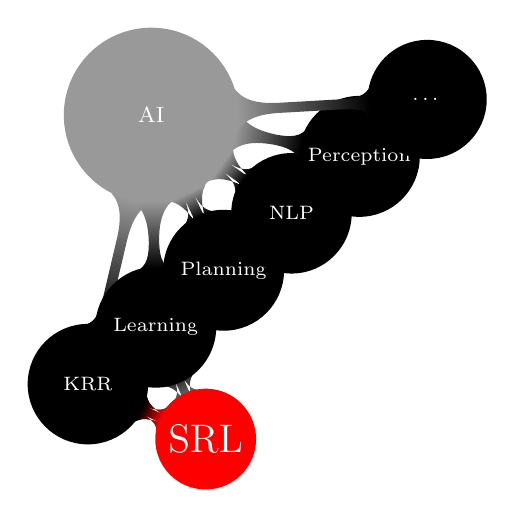
\begin{tikzpicture}[small mindmap, scale=.75]
 \path[mindmap,concept color=black,text=white]

 [root concept/.append style={concept color=black!40,minimum size=1.5cm},
 level 1 concept/.append style={every child/.style={concept color=black!100,minimum size=.7cm, sibling angle=60}},
 level 2 concept/.append style={every child/.style={concept color=red,minimum size=.6cm, sibling angle=60}},
%level 3 concept/.append style={every child/.style={concept color=black!40,minimum size=0.7cm, sibling angle=60}},
 mindmap]
 node[concept]{AI} [clockwise from=0, grow =-50]
 child[]{node[concept,minimum size=1cm] (KRR) {KRR}
   child[grow=-25] {node[concept] (SRL) {\Large SRL}}}
 child[] { node[concept] (ML) {Learning}}
 child[] { node[concept] (Pl) {Planning}}
 child[] { node[concept] {NLP}}
 child[] { node[concept] {Perception}}
 child[] { node[concept] {\dots}};
\begin{pgfonlayer}{background}
 \path (SRL) to[circle connection bar switch color=from (black!60) to (black!80)] (ML);
 \path (SRL) to[circle connection bar switch color=from (black!60) to (black!80)] (KRR);
\end{pgfonlayer}

\end{tikzpicture}
%\caption{The SRL mindmap\label{Fig:SRL-mindmap}}
\end{center}
\end{figure}\vspace{2cm}}
\column{.45\textwidth}{
\begin{block}{Statistical Relational Learning}
 is a subdiscipline of artificial intelligence that is concerned with
 domain models that exhibit both \alert{\bf uncertainty} and \alert{\bf
   complex relational structure}. 
\end{block}}
\end{columns}
\end{frame}

\begin{frame}
  \frametitle{Hybrid domains}
  We are interested in Statistical Relational Learning over
  \underline{\bf hybrid domains}, i.e., domains that are
  characterized by the presence of 
  \begin{itemize}
  \item \color{blue} structured data (categorical/semantic);
  \item \color{red} continuous data (continuous features);
  \end{itemize}
\end{frame}

\begin{frame}
  \frametitle{Hybrid domains}
  \begin{example}[SRL domain]
  \begin{center}
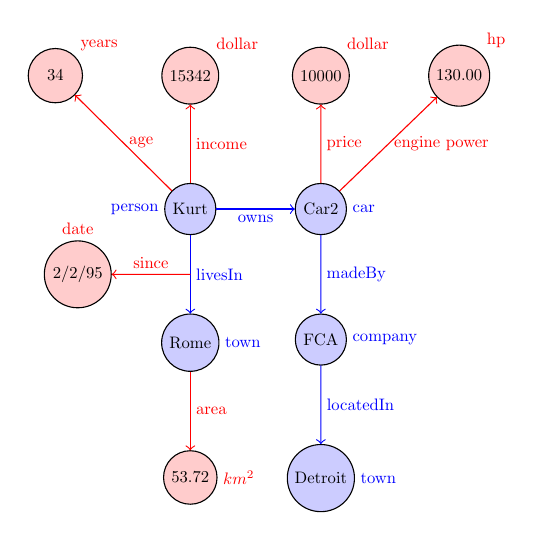
\begin{tikzpicture}[scale=0.6, every node/.style={scale=0.6}]
    \node[fill=blue!20,draw,label=180:{\color{blue}person},circle] (kurt) {Kurt};
    \node[fill=blue!20,label=0:{\color{blue}car},right=of kurt,draw,circle] (car2) {Car2};
    \node[fill=blue!20,label=0:{\color{blue}town},below=of kurt,draw,circle] (rome) {Rome};
    \node[fill=blue!20,label=0:{\color{blue}company},below=of car2,draw,circle] (fca) {FCA};
    \node[fill=blue!20,label=0:{\color{blue}town},below=of fca,draw,circle] (detroit) {Detroit};
    \node[fill=red!20,label=45:{\color{red}dollar},above=of car2,draw,circle] (ioooo) {10000}; 
    \node[fill=red!20,label=45:{\color{red}dollar},above=of kurt,draw,circle] (ivooo) {15342};
    \node[fill=red!20,label=45:{\color{red}hp},right=of ioooo,draw,circle] (ieo) {130.00}; 
    \node[fill=red!20,label=0:{\color{red}$km^2$},below=of rome,draw,circle] (vooo) {53.72};
    \node[fill=red!20,label=45:{\color{red}years},left=of ivooo,draw,circle] (ea) {\ \ 34\ \ \ };
    \draw[->,blue] (kurt) to node[below]{owns} (car2);
    \draw[->,blue] (kurt) to node[right](livesin){livesIn} (rome);
    \draw[->,blue] (car2) to node[right]{madeBy} (fca);
    \draw[->,blue] (fca) to node[right]{locatedIn} (detroit);
    \draw[->,red] (car2) to node[right]{price} (ioooo);
    \draw[->,red] (car2) to node[right]{engine power} (ieo);
    \draw[->,red] (kurt) to node[right]{income} (ivooo);
    \draw[->,red] (kurt) to node[right]{age} (ea);
    \draw[->,red] (rome) to node[right]{area} (vooo); 
    \node[fill=red!20,label=90:{\color{red}date},left=of livesin,draw,circle] (start) {2/2/95};
    \draw[->,red] (livesin) to node[above]{since} (start); 
  \end{tikzpicture}
\end{center}
\end{example}
\end{frame}

\begin{frame}
\frametitle{Tasks in Statistical Relational Learning}
\begin{columns}
  \column{.47\textwidth}
{
  \begin{itemize}
  \item {\color{blue} Object Classification:} Predicting the type of an
    object based on its relations and attributes;
  \item {\color{blue} Reletion detenction:} Predicting if two objects
    are connected by a relation, based on types and attributes of the
    participating objects;
  \item{\color{red} Regression:} predicting the (distribution of) values of the attributies of an object,
    (a pair of related objects) based on the types and relations of the object(s) involved. 
  \end{itemize}}
\column{.5\textwidth}
{
\begin{example}[SRL domain]
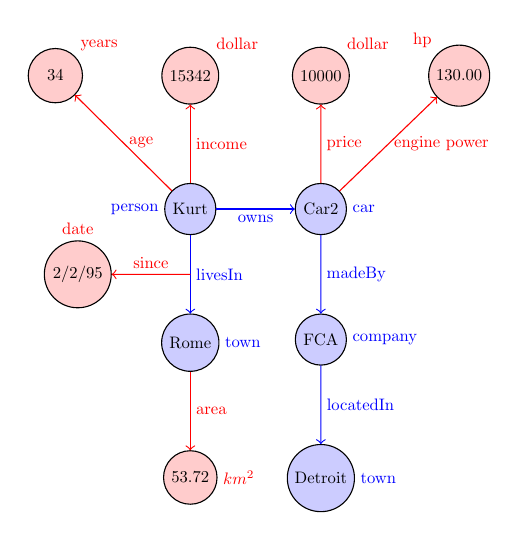
\begin{tikzpicture}[scale=0.6, every node/.style={scale=0.6}]
    \node[fill=blue!20,draw,label=180:{\color{blue}person},circle] (kurt) {Kurt};
    \node[fill=blue!20,label=0:{\color{blue}car},right=of kurt,draw,circle] (car2) {Car2};
    \node[fill=blue!20,label=0:{\color{blue}town},below=of kurt,draw,circle] (rome) {Rome};
    \node[fill=blue!20,label=0:{\color{blue}company},below=of car2,draw,circle] (fca) {FCA};
    \node[fill=blue!20,label=0:{\color{blue}town},below=of fca,draw,circle] (detroit) {Detroit};
    \node[fill=red!20,label=45:{\color{red}dollar},above=of car2,draw,circle] (ioooo) {10000}; 
    \node[fill=red!20,label=45:{\color{red}dollar},above=of kurt,draw,circle] (ivooo) {15342};
    \node[fill=red!20,label=135:{\color{red}hp},right=of ioooo,draw,circle] (ieo) {130.00}; 
    \node[fill=red!20,label=0:{\color{red}$km^2$},below=of rome,draw,circle] (vooo) {53.72};
    \node[fill=red!20,label=45:{\color{red}years},left=of ivooo,draw,circle] (ea) {\ \ 34\ \ \ };
    \draw[->,blue] (kurt) to node[below]{owns} (car2);
    \draw[->,blue] (kurt) to node[right](livesin){livesIn} (rome);
    \draw[->,blue] (car2) to node[right]{madeBy} (fca);
    \draw[->,blue] (fca) to node[right]{locatedIn} (detroit);
    \draw[->,red] (car2) to node[right]{price} (ioooo);
    \draw[->,red] (car2) to node[right]{engine power} (ieo);
    \draw[->,red] (kurt) to node[right]{income} (ivooo);
    \draw[->,red] (kurt) to node[right]{age} (ea);
    \draw[->,red] (rome) to node[right]{area} (vooo); 
    \node[fill=red!20,label=90:{\color{red}date},left=of livesin,draw,circle] (start) {2/2/95};
    \draw[->,red] (livesin) to node[above]{since} (start); 
  \end{tikzpicture}
\end{example}}
\end{columns}
\end{frame}

\begin{frame}\small
\frametitle{Real-world uncertain, structured and hybrid domains}
\begin{tikzpicture}
\node[text width=.55\textwidth] (robotics) {
{\color{violet}\bf Robotics:} a {\color{red}robot's location} is
    a continuous values while the {\color{blue} the types of 
    the objects it encounters} can be described by discrete set of classes};
\node[right=0 of robotics] 
{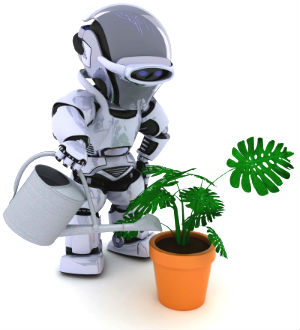
\includegraphics[width=.15\textwidth]{robot.jpg}};
\node[text width=.6\textwidth,below=.3 of robotics] (image) {
  {\color{violet}\bf Semantic Image Interpretation:} The {\color{red}
    visual features} of a bounding box of a picture are continuous values,
  while the {\color{blue} types of objects} contained in a bounding box
  and the {\color{blue} relations between them} are taken from a discrete set};
\node[right=0 of
image]{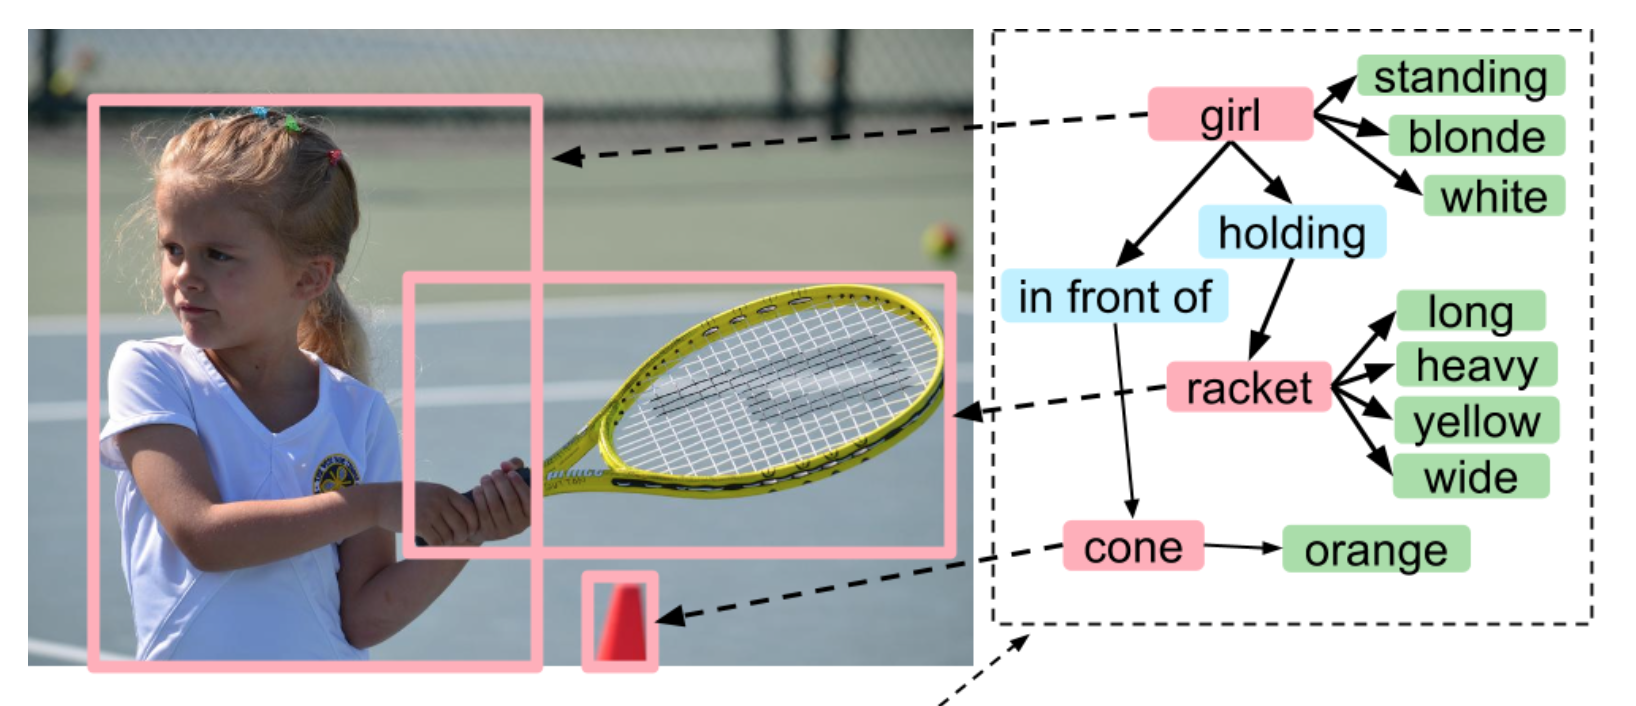
\includegraphics[width=.4\textwidth]{scene_graph.png}};
\node[text width=.6\textwidth,below=.3 of image] (nlp) {
  {\color{violet}\bf Natural Language Processing:} The {\color{red}
  distributional semantics} provide a vectorial (numerical)
representation of the meaning of words, while WordNet associates
  to each word a set of {\color{blue} synsets and a set of relations
    with other words} which are finite and discrete};
\node[right=-.3 of nlp]{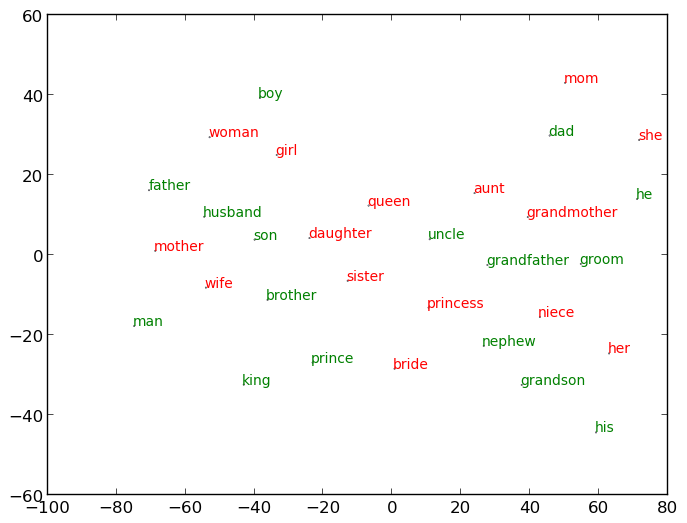
\includegraphics[width=.2\textwidth]{distributional-semantics.png}};
\node[right=2 of nlp]{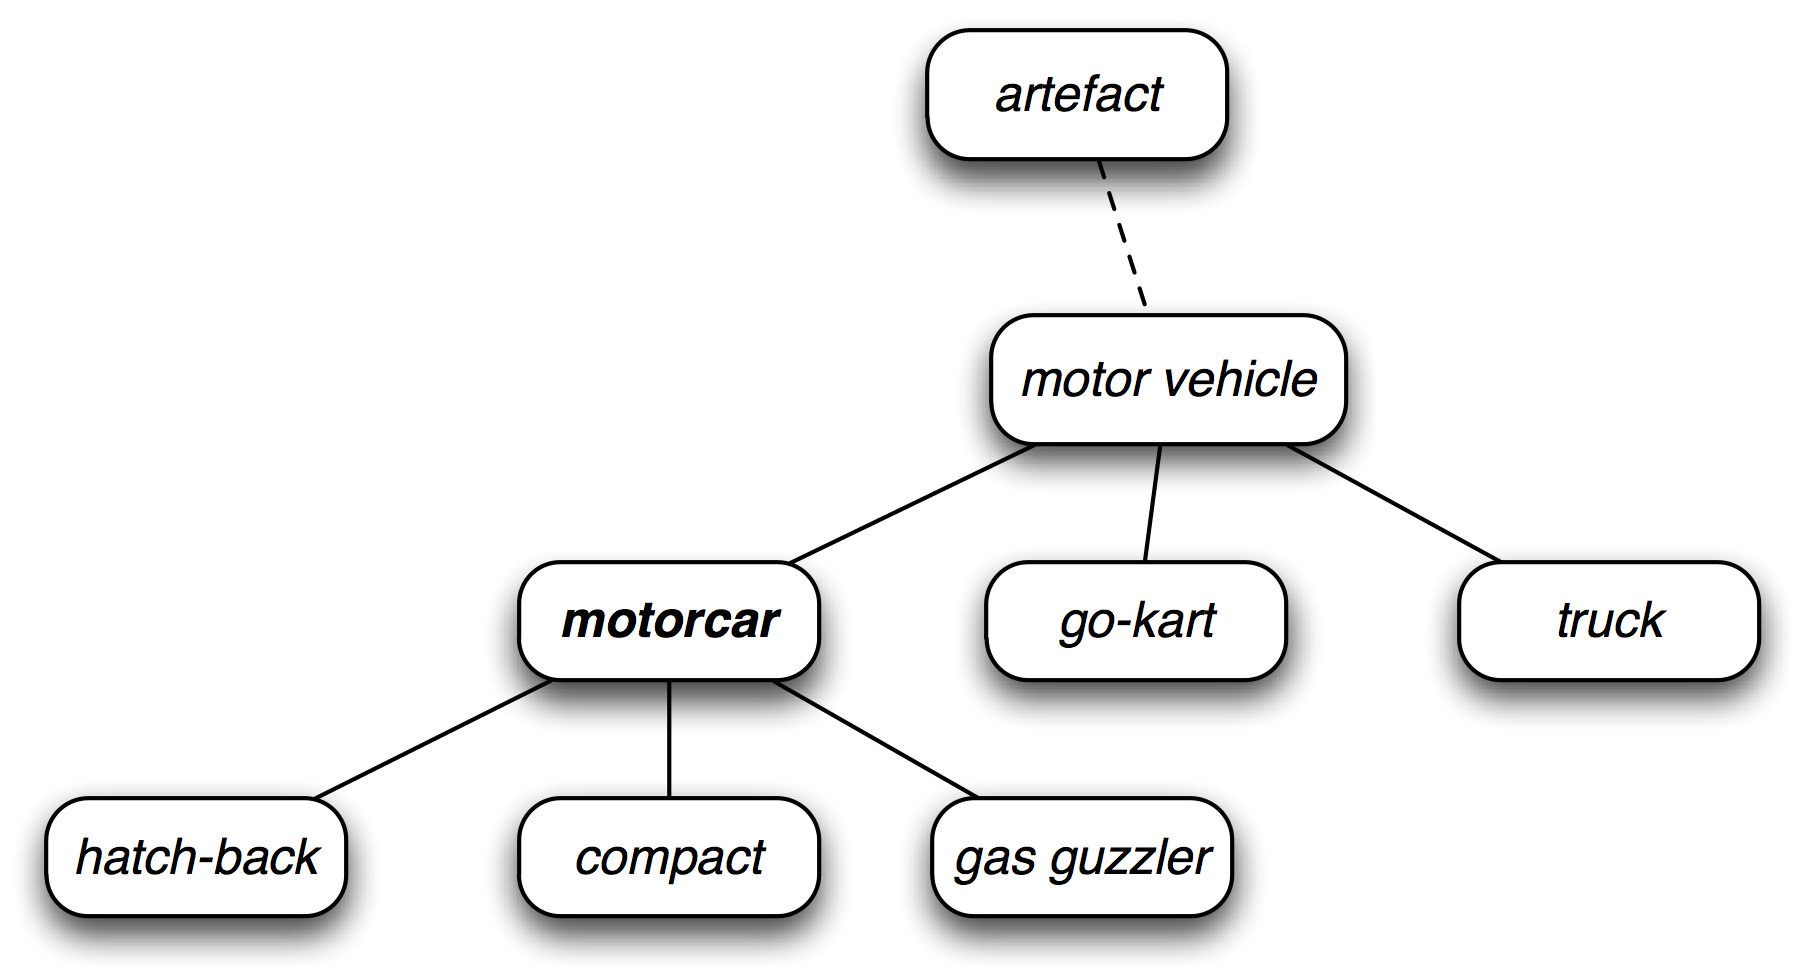
\includegraphics[width=.2\textwidth]{wordnet.png}};
\end{tikzpicture}
\end{frame}

\section{Semantic Image Interpretation}

\begin{frame}
  \frametitle{Semantic Image interpretation}
  \begin{block}{semantic Image Interpretation (SII)}
    \begin{itemize}
    \item<2-> detect the \alert{main objects} shown in the picture;
    \item<3-> assign to each object an \alert{object type};
    \item<4-> determine the \alert{relations} between the objects as shown in
      the picture
    \item<4-> represent the outcome of the detection in a \alert{semantic
      structure}.
    \end{itemize}
  \end{block}
  \begin{tikzpicture}[scale=.8]\footnotesize
    \node (pic) {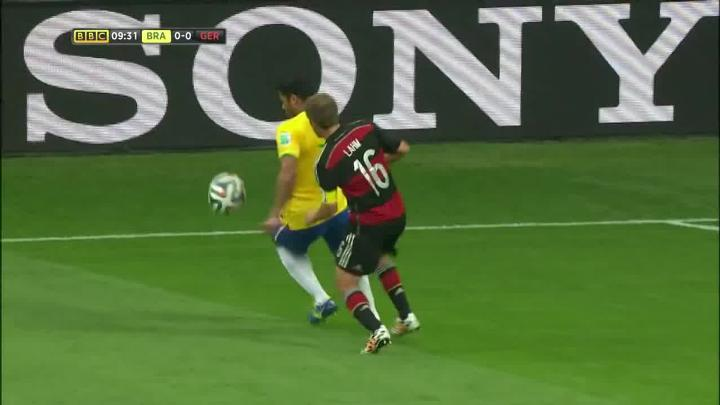
\includegraphics[width=.56\textwidth]{football.jpg}};
    \onslide<2->{\draw[very thick, blue] (-1.9,-.2) rectangle +(.6,.6);
    \draw[very thick, yellow] (-1.2,-1.5) rectangle +(1,3.2);
    \draw[very thick, pink] (-1.1,-1.4) rectangle +(.8,1.2);
    \draw[very thick, red] (-.5,-1.9) rectangle +(1.2,3.2);
    \draw[very thick, magenta] (-.4,-1.9) rectangle +(.7,1.6);
    \draw[very thick, blue!40] (.2,-1.6) rectangle +(.6,1.4);
    \draw[very thick, green] (-0.17,0) rectangle +(.6,.7);
    \draw[very thick, white] (-4,.5) rectangle +(8,1.8);}
    \onslide<3->{
    \draw[very thick, blue] (-1.9,-.2) rectangle
       node[above left] (ballbb) {ball}+(.6,.6);
    \draw[very thick, yellow] (-1.2,-1.5) rectangle
      node[above left] (playerbrbb) {player} +(1,3.2);
    \draw[very thick, pink] (-1.1,-1.4) rectangle
      node[above left] (legplbrbb) {leg} +(.8,1.2);
    \draw[very thick, red] (-.5,-1.9) rectangle 
       node[above right] (playergebb) {player} +(1.2,3.2);
    \draw[very thick, magenta] (-.4,-1.9) rectangle
      node[below] (legplge1bb) {leg} +(.7,1.6);
    \draw[very thick, blue!40] (.2,-1.6) rectangle
      node[right] (legplge2bb) {leg} +(.6,1.4);
    \draw[very thick, green] (-0.17,0) rectangle
       node[above right] (numberbb) {number} +(.6,.7);
    \draw[very thick, white] (-4,.5) rectangle
       node[above right] (sponsorbb) {logo}  +(8,1.8);}
   \onslide<4->{
     \node[draw=black,
	right=.1 of pic,
	circle,
	fill=blue,
	text=white,
	label={ball}](ball){$b_1$};
     \node[draw=black,
	right=.7of ball,
	circle,
	fill=yellow,
	text=black,
	label={player}](playerbr){$b_2$};
     \node[draw=black,
	right=1.5of playerbr,
	circle,
	fill=red,
	text=white,
	label=0:{player}](playerge){$b_3$};
     \node[draw=black,
	below=of playerbr,
	circle,
	fill=pink,
	text=black,
	label=180:{leg}](playerbrleg){$b_4$}; 
     \node[draw=black,
	below left=1 and .2 of playerge,
	circle,
	fill=magenta,
	text=white,
	label=180:{leg}](playergeleg1){$b_5$}; 
     \node[draw=black,
	below right=1 and .2 of playerge,
	circle,
	fill=blue!40,
	text=black,
	label=180:{leg}](playergeleg2){$b_6$}; 
     \node[draw=black,
	above right=.7 and .2of playerge,
	circle,
	fill=green,
	text=black,
	label={number}](number){$b_7$};
     \node[draw=black,
	above=of playerbr,
	circle,
	label=0:{logo}](logo){$b_8$}; 
   \draw[->] (playerbr) -- node[below] {kicks} (ball);
   \draw[->] (playerbrleg) -- node[left] {partOf} (playerbr);
   \draw[->] (playergeleg1) -- (playerge);
   \draw[->] (playergeleg2) -- node[left] {partOf} (playerge);
   \draw[->] (playerge) -- node[left] {hasNum} (number);
   \draw[->] (playerge) -- node[below] {attaks} (playerbr);
 }
   \end{tikzpicture}
 \end{frame}

\subsection{Language}

\begin{frame}
  \frametitle{Language - to specify knowledge about models}
  Two sorted first order language: ({\color{blue}abstract sort} and {\color{red}numeric sort})
      \begin{itemize}
      \item Abstract constant symbols ({\color{blue} $b_1$,$b_2$,\dots,$b_8$});        
      \item Abstract relation symbols ({\color{blue}
          player(x),
          ball(x),
          partOf(x,y),hasNum(x,y)};
      \item Numeric function symbols ({\color{red}
          xBL(x),yBL(x),width(x),height(h)
          area(x),color(x),contRatio(x,y)};
\end{itemize}

COLOR CODE:
\begin{itemize}
  \item \tikz\node[rectangle,fill=blue]{\ \ \ \ \ \ \ \ }; denotes
    objects and relations of the domain structure;
  \item \tikz\node[rectangle,fill=red]{\ \ \ \ \ \ \ \ };  denotes
    attributes and relations between attributes of the numeric part of
    the domain.
  \end{itemize}    
\end{frame}

\begin{frame}\footnotesize
  \frametitle{Domain description and queries}
  \begin{columns}
  \begin{column}[t]{.47\textwidth}
  \begin{example}[Domain descritpion:]
    knowledge about object detection:  \\
    {\color{red}
  $xBL(b_1) = 23$, $yBL(b_1) = 73$, \\
  $width(b_1)=20$, $height(b_1)=21$ \\
  $xBL(b_2) = 45$, $yBL(b_1) = 70$, \\
  $width(b_1)=40$, $height(b_1)=104$ \dots \\
  $contRatio(b_2,b_4)=1.0$,
  $contRatio(b_2,b_5)=0.4$, \dots  \\  }
  \pause

  \hrule 
   partial knowledge about object types and relations 

    {\color{blue} $ball(b_1)$,  $player(b_2)$, $player(b_3)$, \\
    $leg(b_4)$, $leg(b_5)$, $partOf(b_3,b_2)$, \\
    $kicks(b_2,b_1)$, $hasNum(b_3,b_7)$,\dots \\
    \pause}

  \hrule 
    ontological axioms 
 \color{blue}

 $\forall xy. partOf(x,y)\wedge leg(x)\imp player(y)$, \\
 $\forall xy, kick(x,y)\imp player(x)\wedge ball(y)$, \\
 $\forall xy partOf(x,y)\imp{\color{red} contRatio(x,y) > .9}$\\
 $\forall x player(x) \imp \neg ball(x)$, \\ 
  \end{example}
\end{column}
\pause
\begin{column}[t]{.5\textwidth}
  \begin{block}{Example (Queries)}
    Query about missing knowledge about object tipes and relations
    ${\color{blue} player(b_{10})}
      \left|
        \color{red}
        \begin{array}{l}
          xBL(b_{10}) = 83,\\ yBL(b_{10} = 42, \\
          width(b_{10}=30 \\ \dots
        \end{array}\right.
      $
      
      $\color{blue} partOf(b_{10},b_{11})
        \left|
        \color{red}
        \begin{array}{l}
          xBL(b_{10}) = 83,\\ yBL(b_{10} = 42, \\
          width(b_{10}=30 \\ \dots \\
          xBL(b_{11}) = 83,\\ yBL(b_{11} = 42, \\
          width(b_{11}=30 \\ \dots \\
          contRatio(b_{10},b_{11}) = 0.6 \\
          contRatio(b_{11},b_{10}) = 0.9 \\
          \dots 
        \end{array}\right.
        $
  \end{block}
\end{column}
\end{columns}
\end{frame}

\begin{frame}
  \frametitle{Logic Tensor Network basic idea}
\begin{center}
  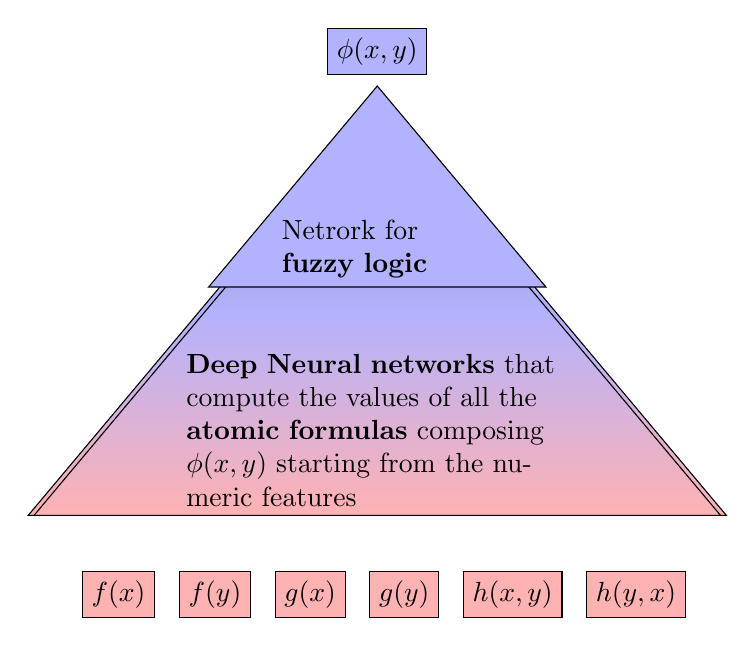
\begin{tikzpicture}[every node/.style={draw,fill=red!30}]
    \node (fx) {$f(x)$};
    \node[right=.3of fx] (fy) {$f(y)$};
    \node[right=.3of fy] (gx) {$g(x)$};
    \node[right=.3of gx] (gy) {$g(y)$};
    \node[right=.3of gy] (hxy) {$h(x,y)$};
    \node[right=.3of hxy] (hyx) {$h(y,x)$};
    \coordinate (half way) at ($ (fx)!0.5!(hyx)$);
    \node[isosceles triangle,
          above=of half way,
          isosceles triangle apex angle=80,
          shape border rotate=90,
          bottom color=red!30,
          top color=blue!30,
          middle color=blue!30, 
          text width=.4\textwidth]
          (LTN)
          {{\bf Logic Tensor Network} that computes the truth value of
          the formula $\phi(x,y)$ on the basis of the numeric features
          of $x$, $y$ and the pair $\left< x, y\right>$};
      \node[fill=blue!30,above=.3of LTN] {$\phi(x,y)$};
      \onslide<2->{
        \node[isosceles triangle,
          above=of half way,
          isosceles triangle apex angle=80,
          shape border rotate=90,
          bottom color=red!30,
          middle color=blue!30,
          text width=.4\textwidth]
          (LTN)
          {{\bf Deep Neural networks} that compute the values of
          all the {\bf atomic formulas} composing $\phi(x,y)$ starting from the numeric features};
        \node[
          isosceles triangle,
          above=3.9of half way,
          isosceles triangle apex angle=80,
          shape border rotate=90,
          fill=blue!30,
          text width=.2\textwidth]
          {Netrork for {\bf fuzzy logic}};}
    \end{tikzpicture}
  \end{center}
\end{frame}

\begin{frame}
  \frametitle{LTN for predicates}
   {\color{red} $n$ unary numeric function
      $f_1(x),\dots,f_n(x)$} and 
{\color{red} $m$ binary numeric function  $g_1(x,y),\dots,g_m(x,y)$}
\begin{block}{LTN for unary predicate/type $\color{blue}P(x)$}
\begin{center}
 \tikz \node[draw,left color=red!20, right color = blue!20] {$LTN_P(\bv) = \sigma\left(u^\intercal_P\tanh\left(\bv^\intercal W_P^{[1:k]}\bv + V_P\bv + b_P\right)\right)$};
\end{center}
$w_P\in\R^{k\times n\times n}$,
$V_P\in\R^{k\times n}$,
$b_P\in\R^{k}$, and 
$u_P\in\R^{k}$ are \underline{\bf parameters}.
\end{block}

\begin{block}{LTN for binary relation $\color{blue}R(x,y)$}
\begin{center}
 \tikz \node[draw,left color=red!20, right color = blue!20] {$LTN_P(\bv) = \sigma\left(u^\intercal_P\tanh\left(\bv^\intercal W_P^{[1:k]}\bv + V_P\bv + b_P\right)\right)$};
\end{center}
$w_P\in\R^{k\times h\times h}$,
$V_P\in\R^{k\times h}$,
$b_P\in\R^{k}$, and 
$u_P\in\R^{k}$ are \underline{\bf parameters}, and  $h=2(n+m)$ = the total number of numeric features that can be
obtained applying $f_i$ and $g_i$ to $x$ and $y$. 
\end{block}
\end{frame}

\begin{frame}
\frametitle{Fuzzy semantics for propositional connectives}
\begin{itemize}
\item In fuzzy semantics {\color{blue} atoms} are assigned with some 
  {\color{red} truth value in real interval [0,1]}
\item connectives have functional semantics. e.g., 
  a binary connective $\circ$ must be interpreted in 
  a function $f_\circ: [0,1]^2\rightarrow [0,1]$. 
\item Truth values are ordeblue, i.e., if $x > y$, then 
   $x$ is a stronger truth than $y$
\item Generalization of classical propositional logic:
\begin{center}
\begin{tabular}{l}
     {\color{blue} $0$ corresponds to FALSE} 
   and \\ {\color{blue} $1$ corresponds to  TRUE}
 \end{tabular}
\end{center}
\end{itemize}
\end{frame}

\begin{frame}
\frametitle{Fuzzy semantics for connectives and quantifiers}
\begin{block}{L{}ukasiewicz T-norm, T-conorm, residual, and precomplement}
\begin{tabular}{llcl}
\color{blue}T-norm & $a\wedge b$ & = & $\max(0,a+b-1)$ \\ \hline \\
\color{blue}T-conorm & $a\vee b$ & = & $\min(1,a+b)$ \\ \\
\color{blue}residual & $a\imp$ &  = & $\left\{
                              \begin{array}{ll} 
                                \mbox{if } a > b & 1-a+b \\ 
                                \mbox{if }a\leq b & 1 
                              \end{array}\right.$ \\ \\
\color{blue}precomplement & $\neg a$ &  = & $1-a$ \\ \\ 
\color{blue}aggregation & $\forall x. a(x)$ & = & 
  $\lim_{n\rightarrow\infty}\left(\frac{1}{n}\sum_{i=1}^n(a(i)^{-1}\right)^{-1}$
\end{tabular}
\end{block}
Alternatively, use G\"odel or Product T-norm, and geometric or
aritmetic mean as aggregator.
\end{frame}

\begin{frame}
\frametitle{Constructive semantics for Existential quantifier}
\begin{itemize}
  \item LTN interprets existential quantifiers constructively via
    Skolemization.
  \item Every formula $\forall x_1,\dots,x_n\exists y \phi(x_1,\dots,x_n,y)$ is
rewritten as
$\forall x_1,\dots,x_m\phi(x_1,\dots,x_n,f(x_1,\dots,x_m))$,
\item 
by introducing a new $m$-ary function symbol $f$,
\end{itemize}
\begin{example}
  $$\forall
  x.(cat(x)\rightarrow\exists y.partof(y,x)\wedge tail(y))$$
  is transformed in 
  $$\forall
  x(cat(x)\rightarrow partOf(tailOf(x),x)\wedge tail(tailOf(x)))$$
\end{example}
\end{frame}

\begin{frame}
\frametitle{Grounding = relation between logical symbols  and data}
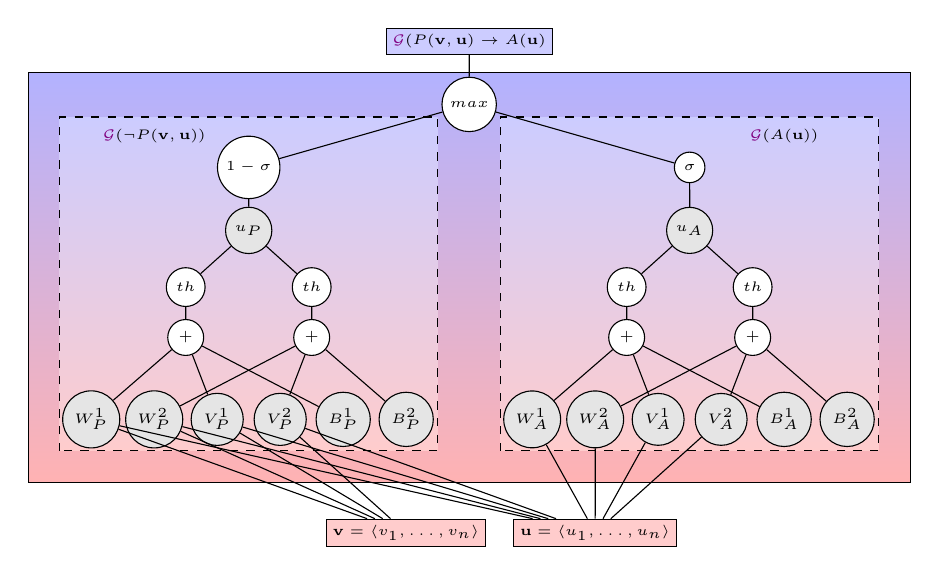
\begin{tikzpicture}[scale=.8]\tiny
\draw[bottom color=red!30, top color=blue!30] (-1,0) rectangle (13,6.5);
\onslide<2>{
\draw[dashed,bottom color=red!20, top color=blue!20] (-.5,.5) rectangle (5.5,5.8);
\draw[dashed,bottom color=red!20, top color=blue!20] (6.5,.5) rectangle (12.5,5.8);
\node at (1,5.5) {$\G(\neg P(\bv,\bu))$};
\node at (11,5.5) {$\G(A(\bu))$};}
\node[rectangle,draw,fill=red!20] (v) at (5,-.8) {$\bv = \left<v_1,\dots,v_n\right>$};
\node[rectangle,draw,fill=red!20] (u) at (8,-.8) {$\bu = \left<u_1,\dots,u_n\right>$};
\node[circle,fill=black!10,draw] (WP1) at (0,1) {$W^1_P$};
\node[circle,fill=black!10,draw] (WP2) at (1,1) {$W^2_P$};
\node[circle,fill=black!10,draw] (VP1) at (2,1) {$V^1_P$};
\node[circle,fill=black!10,draw] (VP2) at (3,1) {$V^2_P$};
\node[circle,fill=black!10,draw] (BP1) at (4,1) {$B^1_P$};
\node[circle,fill=black!10,draw] (BP2) at (5,1) {$B^2_P$};
\node[circle,fill=white,draw] (plusP1) at (1.5,2.3) {$+$};
\node[circle,fill=white,draw] (plusP2) at (3.5,2.3) {$+$};
\node[circle,fill=white,draw] (tanhP1) at (1.5,3.1) {$th$};
\node[circle,fill=white,draw] (tanhP2) at (3.5,3.1) {$th$};
\node[circle,fill=black!10,draw] (UP) at (2.5,4) {$u_P$};
\node[circle,fill=white,draw] (sP) at (2.5,5) {$1-\sigma$};
\draw (v) -- (WP1);
\draw (v) -- (WP2);
\draw (v) -- (VP1);
\draw (v) -- (VP2);
\draw (u) -- (WP1);
\draw (u) -- (WP2);
\draw (u) -- (VP1);
\draw (u) -- (VP2);
\draw (WP1) -- (plusP1); 
\draw (WP2) -- (plusP2); 
\draw (VP1) -- (plusP1);
\draw (VP2) -- (plusP2);
\draw (BP1) -- (plusP1);
\draw (BP2) -- (plusP2);
\draw (plusP1) -- (tanhP1);
\draw (plusP2) -- (tanhP2);
\draw (tanhP1) -- (UP);
\draw (tanhP2) -- (UP);
\draw (UP) -- (sP);
\node[circle,fill=black!10,draw] (WA1) at (7+0,1) {$W^1_A$};
\node[circle,fill=black!10,draw] (WA2) at (7+1,1) {$W^2_A$};
\node[circle,fill=black!10,draw] (VA1) at (7+2,1) {$V^1_A$};
\node[circle,fill=black!10,draw] (VA2) at (7+3,1) {$V^2_A$};
\node[circle,fill=black!10,draw] (BA1) at (7+4,1) {$B^1_A$};
\node[circle,fill=black!10,draw] (BA2) at (7+5,1) {$B^2_A$};
\node[circle,fill=white,draw] (plusA1) at (7+1.5,2.3) {$+$};
\node[circle,fill=white,draw] (plusA2) at (7+3.5,2.3) {$+$};
\node[circle,fill=white,draw] (tanhA1) at (7+1.5,3.1) {$th$};
\node[circle,fill=white,draw] (tanhA2) at (7+3.5,3.1) {$th$};
\node[circle,fill=black!10,draw] (UA) at (7+2.5,4) {$u_A$};
\node[circle,fill=white,draw] (sA) at (7+2.5,5) {$\sigma$};
\draw (u) -- (WA1);
\draw (u) -- (WA2);
\draw (u) -- (VA1);
\draw (u) -- (VA2);
\draw (WA1) -- (plusA1); 
\draw (WA2) -- (plusA2); 
\draw (VA1) -- (plusA1);
\draw (VA2) -- (plusA2);
\draw (BA1) -- (plusA1);
\draw (BA2) -- (plusA2);
\draw (plusA1) -- (tanhA1);
\draw (plusA2) -- (tanhA2);
\draw (tanhA1) -- (UA);
\draw (tanhA2) -- (UA);
\draw (UA) -- (sA);
\node[circle,fill=white,draw] (max) at (6,6) {$max$};
\draw (sP) -- (max);
\draw (sA) -- (max);
\node[rectangle,draw,fill=blue!20] (output) at (6,7) {$\G(P(\bv,\bu)\imp A(\bu)$};
\draw (max) -- (output);
\end{tikzpicture}
\end{frame}
\def\pG{\hat{\G}}
\def\GG{\mathbb{G}}
\begin{frame}
\frametitle{Parameter learning = best satisfiability} 
Given a FOL theory $\K$ the \underline{\textbf{best satisfiability
    problem}} as the problem of finding the set of parameters $\Theta$ of
  the LTN, then the problems become $\G^*=LTN(K,\Theta^*)$
  $$
  \Theta^* = \argmax_{\Theta}\left(\min_{\K\models\phi}LTN(K,\Theta)(\phi)\right)
  $$
\end{frame}

\begin{frame}\footnotesize
  \frametitle{Learning from model description and answering queries}
  \begin{tikzpicture}
    \onslide<2->{\node[rectangle,fill=yellow!20,draw] (learn) {$
     \Theta^* = \argmax_{\Theta}\left(\min_{\K\models\phi}LTN(K,\Theta)(\phi)\right)
     $};}
   \onslide<2->{\node[rotate=45,below left=0 and 0 of learn] (arrowl)
   {
\includegraphics[width=1cm]{arrow.png}};}n
   \onslide<3->{\node[rotate=-45,below right=0 and 0 of learn] (arrowr)
   {
\includegraphics[width=1cm]{arrow.png}};}
   \node[draw,below=.2of arrowl,rectangle,fill=green!20!black!15,label={$\K$}] (kb) 
    {\begin{tabular}{l}
  \color{red} $xBL(b_1) = 23$, $yBL(b_1) = 73$, \\
  \color{red}   $width(b_1)=20$, $height(b_1)=21$ \\
  \color{red} $xBL(b_2) = 45$, $yBL(b_1) = 70$, \\ 
  \color{red} $width(b_1)=40$, $height(b_1)=104$ \dots \\
  \color{red} $contRatio(b_2,b_4)=1.0$,
  \color{red} $contRatio(b_2,b_5)=0.4$, \dots  \\  
  \color{blue}$ball(b_1)$,  $player(b_2)$, $player(b_3)$, \\
  \color{blue}  $leg(b_4)$, $leg(b_5)$, $partOf(b_3,b_2)$, \\
  \color{blue}  $kicks(b_2,b_1)$, $hasNum(b_3,b_7)$,\dots \\
  \color{blue} $\forall xy. partOf(x,y)\wedge leg(x)\imp player(y)$, \\
  \color{blue} $\forall xy, kick(x,y)\imp player(x)\wedge ball(y)$, \\
 \color{blue}  $\forall xy partOf(x,y)\imp{\color{red} contRatio(x,y) > .9}$\\
 \color{blue}  $\forall x player(x) \imp \neg ball(x)$, \\ 
    \end{tabular}};
   \onslide<3->{\node[draw,below=.2of arrowr,rectangle,fill=green!20!black!30,label={$Q$}] (Q) 
   {\begin{tabular}{l}
      $LTN_{K,\Theta^*}\left(
      {\color{blue} player(b_{10})}
      \left|
        \color{red}
        \begin{array}{l}
          xBL(b_{10}) = 83,\\ yBL(b_{10} = 42, \\
          width(b_{10})=30 \\ \dots
        \end{array}\right.\right)$
   \end{tabular}};}
\end{tikzpicture}
\end{frame}

\begin{frame}
  \frametitle{Semantic Image interpretation}
  \begin{block}{semantic Image Interpretation (SII)}
    \begin{itemize}
    \item<2-> object detection: Fast RCNN (state of the art
      object detector)
    \item<3-> Fast-RCNN returns candidate
      bounding boxes, associated with weights for each object class;
    \item<6-> For each pair of bounding boxe we compute additional
      binary feature that measure the mutual overlap between the two
      bounding boxes. 
    \end{itemize}
  \end{block}
  \begin{tikzpicture}[scale=.8]\footnotesize
    \node (pic) {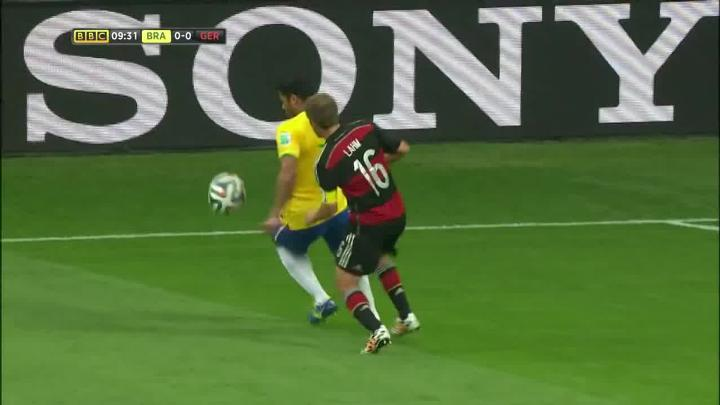
\includegraphics[width=.56\textwidth]{football.jpg}};
    \onslide<2->{\draw[very thick, blue] (-1.9,-.2) rectangle node (ballbb) {} +(.6,.6);
    \draw[very thick, yellow] (-1.2,-1.5) rectangle node (playerbrbb)
    {} +(1,3.2);
    \draw[very thick, pink] (-1.1,-1.4) rectangle node (playergebb) {}
    +(.8,1.2);
    \draw[very thick, red] (-.5,-1.9) rectangle +(1.2,3.2);
    \draw[very thick, magenta] (-.4,-1.9) rectangle +(.7,1.6);
    \draw[very thick, blue!40] (.2,-1.6) rectangle +(.6,1.4);
    \draw[very thick, green] (-0.17,0) rectangle +(.6,.7);
    \draw[very thick, white] (-4,.5) rectangle +(8,1.8);}
  \onslide<3->{
  \node[draw,right=of pic,rectangle,fill=blue!30,text width=.3\textwidth]
  (ballfeatures) 
  {\color{red}$
    \begin{array}{l}
      xBL(b_1) = 12 \\
      yBL(b_1) = 27 \\
      width(b_1) = 30 \\
      height(b_1) = 30 \\
      rcnn_{ball}(b_1) = .8 \\
      rcnn_{player}(b_1) = .3 \\
      rcnn_{logo}(b_1) = .02 \\
      \dots 
    \end{array}$};
  \draw[blue, very thick,->] (ballbb) -- (ballfeatures);}
  \onslide<4->{
  \node[draw,below right=-3 and .7 of pic,rectangle,fill=yellow!30,text width=.3\textwidth]
  (playerbrfeatures) 
  {\color{red}$
    \begin{array}{l}
      xBL(b_1) = 14 \\
      yBL(b_1) = 17 \\
      width(b_1) = 40 \\
      height(b_1) = 100 \\
      rcnn_{ball}(b_1) = .1\\
      rcnn_{player}(b_1) = .7 \\
      rcnn_{logo}(b_1) = .02 \\
      \dots 
    \end{array}$};
  \draw[yellow, very thick,->] (playerbrbb) -- (playerbrfeatures);}
  \onslide<5->{
  \node[draw,below right=-3.4 and 1.3 of pic,rectangle,fill=red!30,text width=.3\textwidth]
  (playergefeatures) 
  {\color{red}$
    \begin{array}{l}
      xBL(b_1) = 34 \\
      yBL(b_1) = 37 \\
      width(b_1) = 44 \\
      height(b_1) = 130 \\
      rcnn_{ball}(b_1) = .1\\
      rcnn_{player}(b_1) = .74 \\
      rcnn_{logo}(b_1) = .1 \\
      \dots 
    \end{array}$};
  \draw[red, very thick,->] (playergebb) -- (playergefeatures);}
  \onslide<6->{
    \node[draw,below right=-.8 and -.3 of pic,rectangle,
    fill=orange!30,
    fill=orange!30,
    text width=.3\textwidth]
  (playersoverlaps) 
  {\color{red}$
    \begin{array}{l}
      contRatio(b_2,b_3) = 0.3 \\
      contRatio(b_3,b_2) = 0.2 
    \end{array}$};
  \draw[red, very thick,->] (playergebb) -- (playersoverlaps);
  \draw[yellow, very thick,->] (playerbrbb) -- (playersoverlaps);}
\end{tikzpicture}
 \end{frame}

\begin{frame}
\frametitle{LTN evaluation on PascalPart dataset}
\begin{itemize}
\item PascalPart contains \textbf{10103 pictures} annotated with a set
  of bounding boxes labelled with object types (60 classes among
  animals, vehicles, and indor objects)   
\item We train an LTN with the approx 2/3 pictures and test on 1/3.
  by including the following \textbf{background knowledge}
  \begin{itemize}
    \item positive/negative examples for object classes (from training set)
      $\color{blue}weel(bb1),\ car(bb2),\ \neg horse(bb2),\neg person(bb4)$

    \item positive/negative examples for relations (we focus on
      parthood relation). {\color{blue} $partOf(bb1,bb2),\ \neg partOf(bb2,bb3),\dots$}
    \item general axioms about parthood relation:
      $\color{blue}\forall x. car(x)\wedge partof(y,y)\imp wheeel(y)\vee mirror(y)
      \vee door(y)\vee \dots) $
    \end{itemize}
\end{itemize}
\end{frame}
\begin{frame}
  \frametitle{LTN for SII results}
  \begin{columns}
    \begin{column}{.4\textwidth}
    \begin{tabular}{l}
    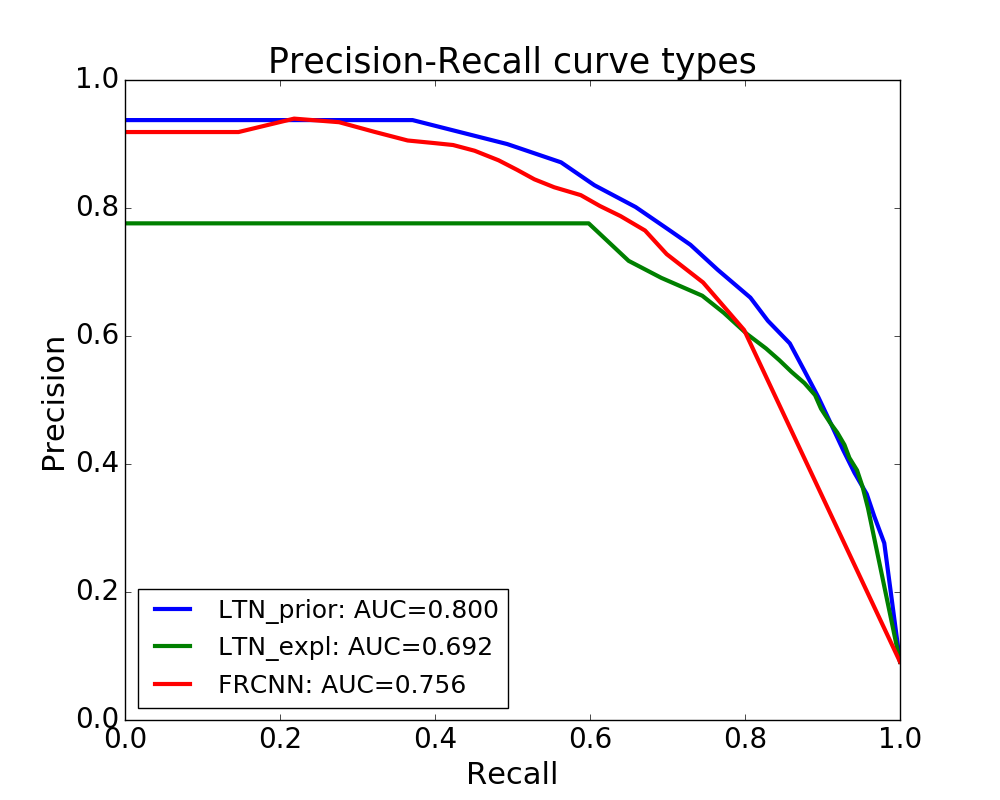
\includegraphics[width=\textwidth]{prec_rec_curve_0_types.png} \\
    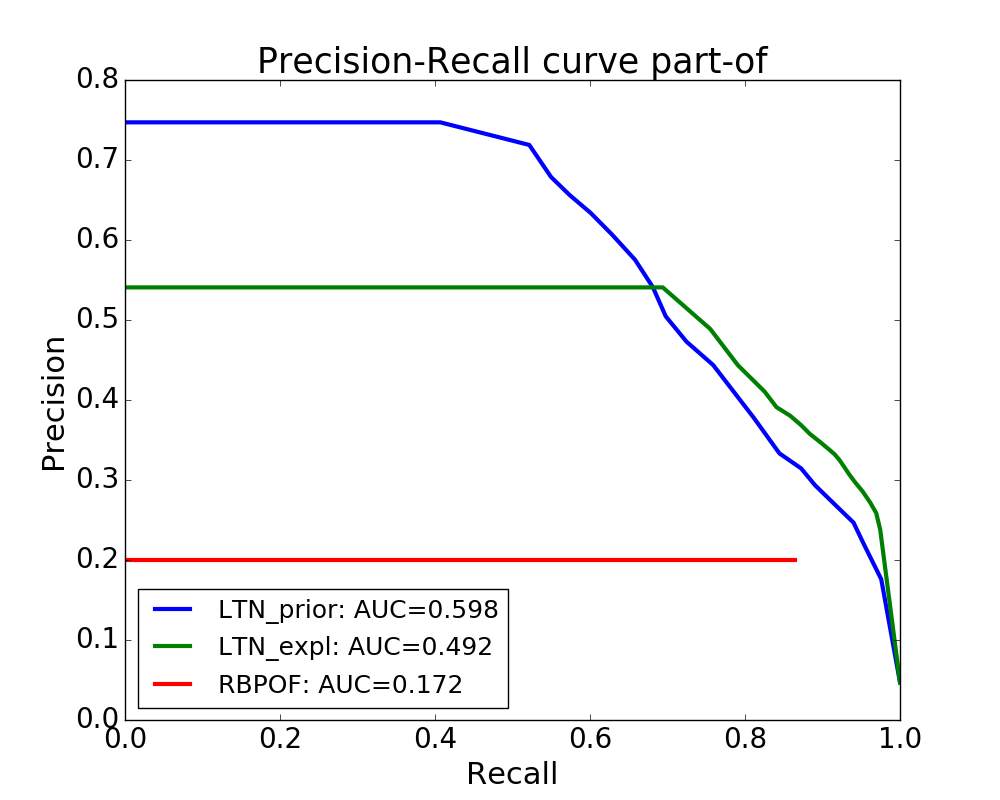
\includegraphics[width=\textwidth]{prec_rec_curve_0_part-of.png}  
    \end{tabular}
  \end{column}
  \begin{column}{.55\textwidth}
    \begin{itemize}
      \item {\color{blue} $LTN_{prior}$ is an LTN trained with
          positive and negative examples + general
            axioms about partOo relation}
      \item {\color{green!50!black} $LTN_{expl}$ is an LTN trained
        only with  positive and negative
          examples of types and partOf}
      \item {\color{red} $FRCNN$ is the baseline proposal
      classification for types given by Fast-RCNN}
      \item {\color{red} $RBPOF$ is the baseline for partOf based
          on the naive criteria
          $$area\  containment \geq threshold$$}
    \end{itemize}
  \end{column}
\end{columns}  
\end{frame}
\begin{frame}
  \frametitle{Robustness w.r.t. noisy data}
  \begin{itemize}
    \item logical axioms improve the robustness of the system in
      presence of noise in the labels of training data.
    \item e artificially add an increasing amount of noise to the
      PascalPart-dataset training data, and we measure the
      degradation of the performance,
      \hspace*{-3em}
      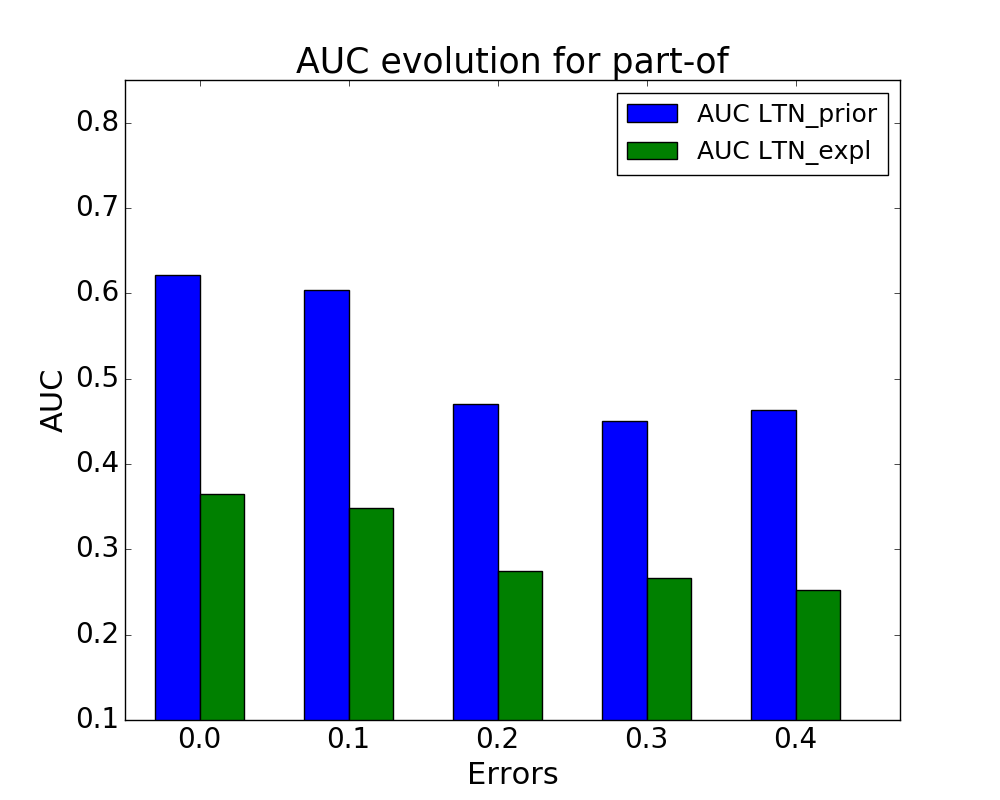
\includegraphics[width=0.5\textwidth]{AP_part-of} 
       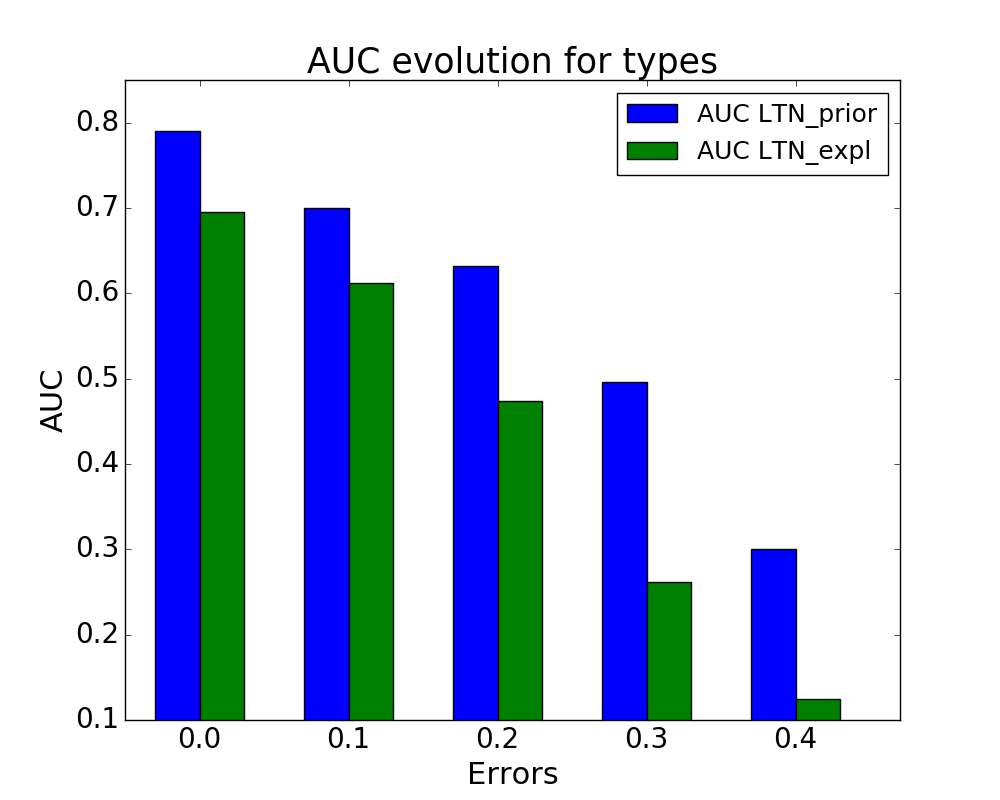
\includegraphics[width=0.5\textwidth]{AP_types}
    \end{itemize}
  \end{frame}  

\begin{frame}
  \frametitle{Conclusions}
  \begin{itemize}
  \item we introduce \textbf{Logic Tensor Networks},
    a general framework for SRL that integrates
      fuzzy logical reasoning and machine learning based on neural networks;
    \item We apply LTN to the challanging problem of \textbf{semantic image
      interpretation};
  \item We experimentally show that the \textbf{usage of
      logic based background knowledge
      improves the performance} of automatic classification based
      only on numeric features.
  \end{itemize}
\end{frame}
\begin{frame}
  \frametitle{Thanks}
  \begin{center}
    \Huge Thanks for your attention 
\end{center}
\end{frame}
\end{document}
